\documentclass[a4paper,11pt]{article}

\usepackage[utf8]{inputenc}
\usepackage[T1]{fontenc}
\usepackage[francais]{babel}
\usepackage{amsmath,amssymb}
\usepackage{fullpage}
\usepackage{xspace}
\usepackage{graphicx}
\usepackage{verbatim}
\usepackage{listings}
\usepackage[usenames,dvipsnames]{color}
\usepackage{url}
\usepackage{mdframed}   % AJOUT
\usepackage{xcolor}     % AJOUT
\usepackage{float}      % AJOUT
\usepackage{stmaryrd}   % AJOUT
\usepackage{ntheorem}   % AJOUT
\usepackage[french]{algorithm2e}    % AJOUT

\lstset{basicstyle=\small\tt,
  keywordstyle=\bfseries\color{Orchid},
  stringstyle=\it\color{Tan},
  commentstyle=\it\color{LimeGreen},
  showstringspaces=false}

\newtheorem{question}{Question}
\newtheorem{exo}{Exercice}

\newcommand{\dx}{\,dx}
\newcommand{\ito}{,\dotsc,}
\newcommand{\R}{\mathbb{R}}
\newcommand{\C}{\mathbb{C}}
\newcommand{\N}{\mathbb{N}}
\newcommand{\Poly}[1]{\mathcal{P}_{#1}}
\newcommand{\abs}[1]{\left\lvert#1\right\rvert}
\newcommand{\norm}[1]{\left\lVert#1\right\rVert}
\newcommand{\pars}[1]{\left(#1\right)}
\newcommand{\bigpars}[1]{\bigl(#1\bigr)}
\newcommand{\set}[1]{\left\{#1\right\}}

% Personnalisation pour le TP
\newcommand{\quest}[1]{\small\textbf{#1}\normalsize}
\setlength{\parindent}{0pt}
\newcommand*\biggestpart{}

\newenvironment{sbmatrix}[1]
 {\def\mysubscript{#1}\mathop\bgroup\begin{bmatrix}}
 {\end{bmatrix}\egroup_{\textstyle\mathstrut\mysubscript}}

\theoremstyle{nonumberplain}
\newmdtheoremenv[%
  backgroundcolor=gray!10,
  linecolor=gray!75,
  linewidth=2pt,
  topline=false,
  rightline=false,
  bottomline=false]{calculs}{}

\theoremstyle{nonumberplain}
\newmdtheoremenv[%
  backgroundcolor=blue!10,
  linecolor=blue!75,
  linewidth=2pt,
  topline=false,
  rightline=false,
  bottomline=false]{ref_scilab}{}

\theoremstyle{nonumberplain}
\newmdtheoremenv[%
  backgroundcolor=purple!10,
  linecolor=purple!75,
  linewidth=2pt,
  topline=false,
  rightline=false,
  bottomline=false]{proposition}{}

\title{Compte-rendu en \textit{Méthodes numériques de base} \\
\textbf{Résultats sur l'identification de conductivité}}
\author{Aurélien PEPIN, Antonin KLOPP-TOSSER}
\date{2 mai 2017}

% ===============
\begin{document}

\maketitle

\section{Méthode des différences finies}

    \quest{QUESTION 1}. L'écriture sous forme matricielle du $\theta$-schéma \textit{(10)} exprime l'itération $k + 1$ du vecteur $U$ en fonction de l'itération $k$.
    On isole donc, dans le $\theta$-schéma, les termes en $u_{i}^{(k + 1)}$.

    \begin{calculs}
        \begin{alignat*}{3}
            & & & u_{i}^{(k + 1)} - \mu\theta\left(C_{i + 1/2}\,u_{i + 1}^{(k + 1)} - (C_{i + 1/2} + C_{i - 1/2})\,u_{i}^{(k + 1)} + C_{i - 1/2}\,u_{i - 1}^{(k + 1)}\right) \\
            & & & = \mu(1 - \theta)\left(C_{i + 1/2}\,u_{i + 1}^{k} - (C_{i + 1/2} + C_{i - 1/2})\,u_{i}^{k} + C_{i - 1/2}\,u_{i - 1}^{k}\right) + u_{i}^{k} \\
            & & & \\
            & \iff & & \left(1+\theta\mu(C_{i + 1/2} + C_{i - 1/2})\right)\,u_{i}^{(k + 1)} - \theta\mu(C_{i + 1/2}\,u_{i + 1}^{(k + 1)}) - \theta\mu(C_{i - 1/2}\,u_{i - 1}^{(k + 1)}) \\
            & & & = \left(1 + (\theta - 1)\mu(C_{i + 1/2} + C_{i - 1/2})\right)\,u_{i}^{k} - (\theta - 1)\mu\,C_{i + 1/2}\,u_{i + 1}^{k} - (\theta - 1)\mu\,C_{i - 1/2}\,u_{i - 1}^{k}
        \end{alignat*}
    \end{calculs}

    \medskip
    Sachant que $U^{(k)}$ est la matrice-colonne des $u_{i}^{(k)}$ $\forall i \in \llbracket 1; n \rrbracket$, on identifie
    les termes un à un dans le membre de gauche puis dans le membre de droite :

    \begin{calculs}
        $$
        \left(
            I + \theta\mu
            \noindent
            \resizebox{0.60\linewidth}{!}{%
                $\begin{bmatrix}
                    C_{1 + 1/2} + C_{1 - 1/2} & -C_{1 + 1/2} & & 0\\
                    -C_{2 - 1/2} & \ddots & \ddots &  \\
                    & \ddots & \ddots &  -C_{(n - 1) + 1/2} \\
                    0 &  & -C_{n - 1/2} & C_{n + 1/2} + C_{n - 1/2}
                \end{bmatrix}$%
            }
        \right)
        \begin{bmatrix}
            u_{1}^{(k + 1)} \\
            u_{2}^{(k + 1)} \\
            \vdots \\
            u_{n}^{(k + 1)} \\
        \end{bmatrix}
        $$
        \hspace{42ex} A \hspace{30ex} $U^{(k + 1)}$
    \end{calculs}
    \begin{calculs}
        $$
        \left(
            I + (\theta - 1)\mu
            \noindent
            \resizebox{0.60\linewidth}{!}{%
                $\begin{bmatrix}
                    C_{1 + 1/2} + C_{1 - 1/2} & -C_{1 + 1/2} & & 0\\
                    -C_{2 - 1/2} & \ddots & \ddots &  \\
                    & \ddots & \ddots &  -C_{(n - 1) + 1/2} \\
                    0 &  & -C_{n - 1/2} & C_{n + 1/2} + C_{n - 1/2}
                \end{bmatrix}$%
            }
        \right)
        \begin{bmatrix}
            u_{1}^{(k)} \\
            u_{2}^{(k)} \\
            \vdots \\
            u_{n}^{(k)} \\
        \end{bmatrix}
        + \mu
        \begin{bmatrix}
            B_1^{(k)} \\
            0 \\
            \vdots \\
            0 \\
        \end{bmatrix}
        $$
        \hspace{42ex} A \hspace{27ex} $U^{(k)}$ \hspace{6ex} $B^{(k)}$
    \end{calculs}

    $B_{1}^{(k)}$ exprime les conditions aux limites. Pour $i = 1$, le terme $(A)_{i, i - 1} = (A)_{1, 0}$
    n'est pas défini et vaut $0$ par convention. Pour conserver l'égalité, on ajoute dans $B$ un coefficient simulé :

      $$ B_1^{(k)} = C_{1/2}\ (\theta\;u_0(t_k) + (1-\theta)\;u_0(t_k+1)) $$

    \newpage
    \quest{QUESTION 2}. Une matrice $M$ est dite définie positive si, pour toute matrice-colonne non nulle $x$ à coefficients réels, $^txMx > 0$.
    Soit $x = (x_1, x_2, ... , x_n)$ non nul :

    \begin{calculs}
      \begin{equation*}
      \begin{split}
          ^txAx   & = \sum\limits_{i = 1}^{n} (C_{i+1/2} + C_{i-1/2}) x_i^2\ -\ 2 \sum\limits_{i = 1}^{n-1}C_{i+1/2}\ x_i\ x_{i+1}
      \end{split}
      \end{equation*}
      {\normalfont On pose} $j = i - 1$ {\normalfont en développant le premier terme :}
      \begin{equation}
      \begin{split}
          ^txAx   & = \sum\limits_{i = 1}^{n} C_{i+1/2}\ x_i^2 + \sum\limits_{j = 0}^{n-1} C_{j+1/2}\ x_{j+1}^2  - 2 \sum\limits_{i = 1}^{n-1} C_{i+1/2}\ x_i\ x_{i+1} \\
                  & = \sum\limits_{i = 1}^{n-1} C_{i+1/2} (x_i - x_{i+1})^2 + C_{1/2}\ x_{1/2}^2 + C_{n + 1/2}\ x_{n}^2 \\
      \end{split}
      \end{equation}
      {\normalfont La fonction} $C(x)$ {\normalfont est strictement positive par définition donc}
      $^txAx > 0\ \forall x$ {\normalfont non nul}.\newline
      {\normalfont La matrice $A$ est bien définie positive.}
    \end{calculs}

\smallskip
\section{Factorisation de Cholesky dans le cas tridiagonal}

    \quest{QUESTION 3}. Phase de factorisation de Cholesky.
    \begin{ref_scilab}
        \raisebox{-0.5ex}{
\includegraphics[height=12px]{images/logo_scilab.png}}
        \emph{Se référer à :} \texttt{\emph{Q3\_Factorisation\_Cholesky.sce}}
    \end{ref_scilab}
    La décomposition de Cholesky permet ensuite de résoudre des systèmes
    linéaires en une phase de descente puis une phase de remontée.

    \bigskip
    \quest{QUESTION 4}. Première phase de descente.
    \begin{ref_scilab}
        \raisebox{-0.5ex}{
\includegraphics[height=12px]{images/logo_scilab.png}}
        \emph{Se référer à :} \texttt{\emph{Q4\_Descente\_Cholesky.sce}}
    \end{ref_scilab}

    \bigskip
    \quest{QUESTION 5}. Seconde phase de remontée.
    \begin{ref_scilab}
        \raisebox{-0.5ex}{
\includegraphics[height=12px]{images/logo_scilab.png}}
        \emph{Se référer à :} \texttt{\emph{Q5\_Remontee\_Cholesky.sce}}
    \end{ref_scilab}

    On peut appliquer dans l'ordre ces trois fonctions pour résoudre l'exemple ci-dessous, noté $MX = B$.
    Le TD 5 a montré que la matrice $M$ était aussi symétrique définie positive
    donc elle admet une unique factorisation de Cholesky.

      \[
      \begin{pmatrix}
          1   &   -1    &   0     &   0     &   0   \\
          -1  &   2     &   -1    &   0     &   0   \\
          0   &   -1    &   2     &   -1    &   0   \\
          0   &   0     &   -1    &   2     &   -1  \\
          0   &   0     &   0     &   -1    &   2   \\
      \end{pmatrix}
      \begin{pmatrix}
          x_1 \\
          x_2 \\
          x_3 \\
          x_4 \\
          x_5 \\
      \end{pmatrix}
      =
      \begin{pmatrix}
          10 \\
          20 \\
          30 \\
          40 \\
          50 \\
      \end{pmatrix}
      \text{ où la solution est }
      X =
      \begin{pmatrix}
          350 \\
          340 \\
          310 \\
          250 \\
          150 \\
      \end{pmatrix}
      \]

    \begin{ref_scilab}
        \raisebox{-0.5ex}{
\includegraphics[height=12px]{images/logo_scilab.png}}
        \emph{Pour calculer et vérifier cet exemple, cf.} \texttt{\emph{Q5\_Exemple\_Cholesky.sce}}
    \end{ref_scilab}

\section{Problème stationnaire}

    \quest{QUESTION 6}. L'équation $(9)$ de l'énoncé fournit une appromixation du système $(13)$ :
        $$ \frac{\partial }{\partial x} [C(x)\frac{\partial u }{\partial x}](x_i, t_k) \approx \frac{C_{i+1/2}\ u_{i+1}^{(k)} - (C_{i+1/2} + C_{i-1/2})\ u_i^{(k)} + C_{i-1/2}\ u_{i-1}^{(k)}}{\delta_x^2} $$

    En écrivant ce système sous forme matricielle pour tout $\forall i \in \llbracket 1; n \rrbracket$, on obtient :
    \begin{calculs}
        $$ \frac{\partial }{\partial x} [C(x)\frac{\partial u }{\partial x}] = \frac{1}{\delta_{x}^2} (-A u + B) = 0
        \iff
        A u = B
        $$
    \end{calculs}

    où, par identification :
    \begin{itemize}
        \item $A$ est la matrice tridiagonale, symétrique et définie positive de la \quest{question 1} ;
        \item $u$ est la matrice-colonne des $u_i^{(k)}$ à l'itération $k$ ;
        \item $B$ est la matrice-colonne des conditions aux limites déterminée de la façon suivante :
    \end{itemize}

    \bigskip
    \textbf{Pour }$\mathbf{i = 1}$.
    \begin{calculs}
        $\begin{aligned}[t]
            (Au)_{1} & = -C_{3/2}\ u_{2}^{(k)} + (C_{3/2} + C_{1/2})\ u_1^{(k)} \\
                     &\iff (B)_{1} = C_{1/2}\ u_{0}
        \end{aligned}$
    \end{calculs}

    \smallskip
    \textbf{Pour }$\mathbf{i > 1}$.
    \begin{calculs}
        $\begin{aligned}[t]
            (Au)_{i} & = -C_{i+1/2}\ u_{i+1}^{(k)} + (C_{i+1/2} + C_{i-1/2})\ u_i^{(k)} - C_{i-1/2}\ u_{i-1}^{(k)} \\
                     & = \frac{\delta_{x}^2}{\delta_{x}^2} (-C_{i+1/2}\ u_{i+1}^{(k)} + (C_{i+1/2} + C_{i-1/2})\ u_i^{(k)} - C_{i-1/2}\ u_{i-1}^{(k)}) \\
                     & \simeq \delta_{x}^2 \cdot 0 \\
                     &\iff (B)_{i} = 0\ \forall i \in \llbracket 2; n \rrbracket
        \end{aligned}$
    \end{calculs}

    La matrice-colonne $B$ est celle de la \quest{question 1} avec la fonction $u_0$ constante.\newline\newline
    Puisque $A$ est définie positive, elle n'admet pas $0$ comme valeur propre.\newline
    Elle est donc inversible et le système $A u = B$ possède par conséquent une unique solution.\newline

    \bigskip
    \quest{QUESTION 7}. Solution exacte du problème stationnaire et convergence.
    \begin{ref_scilab}
        \raisebox{-0.5ex}{
\includegraphics[height=12px]{images/logo_scilab.png}}
        \emph{Se référer à :} \texttt{\emph{Q7\_Probleme\_stationnaire.sce}}
    \end{ref_scilab}

    % On résout l'équation $\forall x \in\ ]-l; l[$ :
    % $$
    % \begin{cases}
    %     \displaystyle
    %     \frac{\partial}{\partial x}[C(x)\frac{\partial u}{\partial x}] = 0 \\
    %     u(-l) = u_0 \\
    %     u(l) = 0
    % \end{cases}
    % $$
    \vspace{-2ex}

    \begin{calculs}
        \vspace{-2ex}
        \begin{equation*}
        \begin{split}
            \frac{\partial}{\partial x}[C(x)\frac{\partial u}{\partial x}] = 0 & \iff
            -\frac{1}{l} \exp(-\frac{x}{l})\ \frac{\partial u}{\partial x} + \exp(-\frac{x}{l})\ \frac{\partial^2 u }{\partial x^2} = 0 \\
            & \iff \frac{\partial^2 u}{\partial x^2} - \frac{1}{l} \frac{\partial u}{\partial x} = 0
        \end{split}
        \end{equation*}
        \emph{donc }$u(x)$\emph{ est de la forme :}
        $$ u(x) = \alpha + \beta \exp(\frac{x}{l}) $$
    \end{calculs}

    \newpage\textbf{Détermination des constantes }$\mathbf{\alpha}$\textbf{ et }$\mathbf{\beta}$.
    \`A partir des conditions initiales, on résout :

    \begin{calculs}
        $$
        \begin{cases}
            u(-l) = \alpha + \beta e^{-1} = u_0 = 1 \\
            u(l) = \alpha + \beta e = 0
        \end{cases}
        \iff
        \begin{cases}
          \beta = \frac{1}{e^{-1} - e} \\
          \alpha = -\frac{e}{e^{-1} - e}
        \end{cases}
        $$
    \end{calculs}

    \medskip
    Finalement, la solution exacte de l'équation différentielle $(13)$ est :

    \begin{calculs}
        $$ u(x) = -\frac{e}{e^{-1} - e} + \frac{1}{e^{-1} - e} \exp(\frac{x}{l}) = \frac{e(e - e^{\frac{x}{l}})}{e^2 - 1}$$
    \end{calculs}

    \medskip
    Il est possible de mesurer la précision de la méthode des différences finies
    en comparant cette solution exacte avec la solution approchée pour
    différents pas $\delta_x \rightarrow 0$.

    \begin{center}
        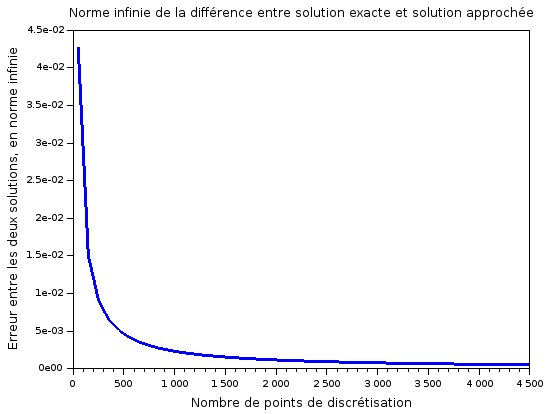
\includegraphics[scale=0.68]{images/q7_ps3.png}
    \end{center}

    Plus le nombre de points de discrétisation $x_{i}$ augmente, plus le pas $\delta_{x}$ tend vers $0$.
    La solution numérique converge vers la solution exacte quand $\delta_x \rightarrow 0$.

\smallskip
\section{\'{E}volution d'une donnée initiale}

    \quest{QUESTION 8}. On cherche à montrer que $\rho(M^{-1}N)$ est strictement inférieur à $1$.
    On applique pour cela à $M^{-1}$ et à $N$ le résultat suivant, démontré plus bas.
    \begin{proposition}
        \hspace{-1ex}\emph{\textbf{Proposition}. Soit $P$ un polynôme d'endomorphisme
        (ou de matrice), soit $S$ une matrice. Si $v$ est vecteur propre de $S$ pour
        la valeur propre $\lambda$, alors il est vecteur propre de $P(S)$ pour la valeur $P(\lambda)$}.
    \end{proposition}

    Soient $P$ et $Q$ deux polynômes de matrice. Dire en effet que $v$ est
    vecteur propre de $S$ associé à la valeur propre $\lambda$ revient à écrire :

    \begin{equation*}
    \begin{split}
        S v = \lambda v & \iff S^{p}\ v = S^{p - 1} \cdot Sv = S^{p - 1} \cdot \lambda v = \lambda^{p} v \quad\forall p \in \mathbb{N} \\
                        & \iff P(S)v = \sum\limits_{k = 0}^{p} a_k\;S^k(v) = \sum\limits_{k = 0}^{p} a_k\;\lambda^kv = P(\lambda)v \\
                        & \iff P^{-1}(S)v = \frac{1}{P(\lambda)}v \\
                        & \iff P^{-1}(S)\ Q(S)v = \frac{Q(\lambda)}{P(\lambda)}v
    \end{split}
    \end{equation*}

    \smallskip
    Soit $x_A$ un vecteur propre de $A$ et $\lambda_A$ sa valeur propre associée.\newline
    $M^{-1}$ et $N$ peuvent être exprimés comme des polynômes de matrice :
    \begin{calculs}
        \vspace{-2ex}
        \begin{equation*}
        \begin{split}
            M^{-1}  = \theta\mu A + I & \iff M^{-1}(A) = \theta\mu A^1 + A^0 \\
            N       = (\theta - 1)\mu A + I & \iff N(A) = (\theta - 1)\mu A^1 + A^0
        \end{split}
        \end{equation*}
        \emph{On en déduit donc la forme des valeurs propres de $M$ et de $N$
        en fonction de celles de A :}
        $$ \lambda_M = 1+\theta \mu \lambda_A\qquad\text{\emph{et}}\qquad\lambda_N = 1+(\theta - 1)\mu \lambda_A$$
        \emph{Les valeurs propres de $M^{-1}N$ sont donc de la forme :}
        $$ \frac{\lambda_N}{\lambda_M} = \frac{1+(\theta - 1)\mu \lambda_A}{1+\theta \mu \lambda_A}
                                       = \frac{1+\theta\mu \lambda_A - \mu \lambda_A}{1+\theta \mu \lambda_A}$$
        \emph{Or, $\mu > 0$ et $A$ est définie positive donc $\lambda_A > 0$, d'où $\mu\lambda_A > 0$.\newline
        Le quotient est donc strictement inférieur à 1.}\newline\newline
        \emph{De plus, $\theta \in [0; 1]$ donc le quotient est toujours strictement supérieur à 1.}
    \end{calculs}

    Toutes les valeurs propres de $M^{-1}N$ sont comprises dans
    l'intervalle $]-1; 1[$ donc :
    $$\rho(M^{-1}N) = \max_i |\lambda_i| < 1$$

    \bigskip
    \quest{QUESTION 9}. D'après le chapitre 3 du cours, la méthode de Crank-Nicolson
    converge si et seulement si $\rho(M^{-1}N) < 1$. La \textbf{question 8}
    a montré que c'était le cas.\newline

    \medskip
    Soit $X$ la limite des $U^{(k)}$. Pour $k \rightarrow +\infty$, on a :
    \begin{calculs}
        \vspace{-2ex}
        \begin{equation*}
        \begin{split}
            MX = NX + \mu B & \iff (M - N) X = \mu B \\
                            & \iff (I + \theta \mu A - I - (\theta - 1) \mu A) X = \mu B \\
                            & \iff \mu A X = \mu B \\
                            & \iff A X = B
        \end{split}
        \end{equation*}
    \end{calculs}

    $A$ et $B$ sont les matrices de la \textbf{question 6} donc la solution
    discrétisée converge bien vers la solution stationnaire.

    \newpage\quest{QUESTION 10}. Dans le graphique ci-dessous, on trace en bleu la solution
    stationnaire trouvée dans la \textbf{question 6}. Puis on trace en
    rouge la solution approchée à différents pas $t_k$.

    \begin{ref_scilab}
        \raisebox{-0.5ex}{
\includegraphics[height=12px]{images/logo_scilab.png}}
        \emph{Se référer à :} \texttt{\emph{Q10\_CrankNicolson.sce}}
    \end{ref_scilab}

    \smallskip
    On choisit les paramètres suivants :
    \begin{itemize}
        \item $n = 100$, nombre de points de discrétisation de la grille ;
        \item $n_t = 6000$, nombre d'itérations assez grand pour approcher de près la solution exacte ;
        \item $T = 500$, ce qui donne un pas de temps $\delta_t \simeq 0.083$.
    \end{itemize}

    \begin{center}
        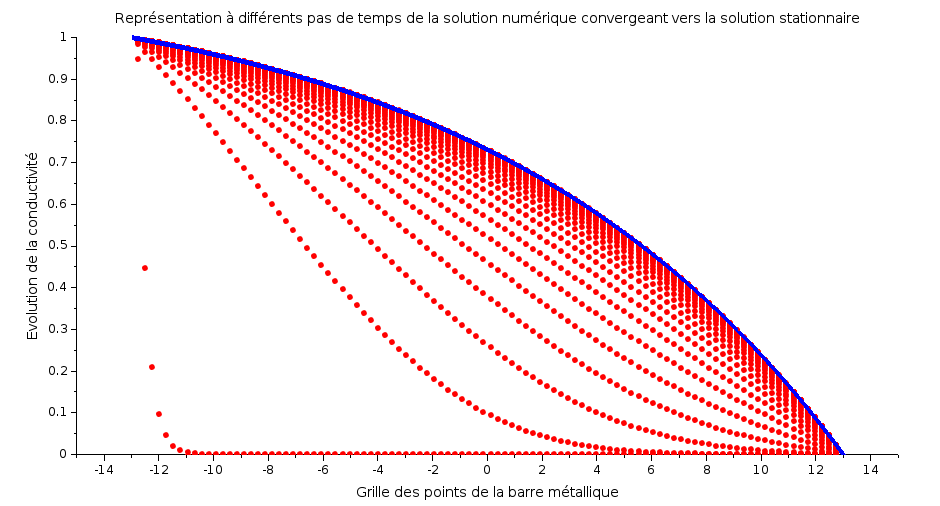
\includegraphics[scale=0.5]{images/q10_approche2.png}
    \end{center}

    Quand $k \rightarrow +\infty$, $U^{(k)}$ tend effectivement vers la solution stationnaire.
    La convergence de la méthode de Crank-Nicolson est rapide : sur le
    graphique, la deuxième mesure, déjà éloignée de $U^{(0)}$, a été relevée à $k = 200$. Chaque courbe rouge
    correspond à $200$ itérations supplémentaires.

\medskip
\section{\'{E}tude du problème inverse}

    \quest{QUESTION 11}. Mesure du flux à $t_{inter} = \frac{2}{3} T$ et $t_{fin} = T$.
    \begin{ref_scilab}
        \raisebox{-0.5ex}{
\includegraphics[height=12px]{images/logo_scilab.png}}
        \emph{Se référer à :} \texttt{\emph{Q11\_Flux.sce}}
    \end{ref_scilab}

    La fonction \texttt{flux(x\_d)} est gourmande en temps.
    Sa complexité temporelle est en $O(n_t \cdot n)$ mais elle cache trois
    étapes en $O(n)$ : le calcul du second membre, la descente et la remontée.

    \medskip
    On en optimise pour cela quelques parties comme le calcul du vecteur $B^{(k)}$ ramené
    au calcul de sa seule composante non nulle $B_1^{(k)}$. On économie ainsi de l'espace mémoire
    et $n$ itérations pour l'affectation.

    \newpage\quest{QUESTION 12}. Recherche de $x_d^{*}$ avec la fonction $J$.
    \begin{ref_scilab}
        \raisebox{-0.5ex}{
\includegraphics[height=12px]{images/logo_scilab.png}}
        \emph{Se référer à :} \texttt{\emph{Q12\_Fonction\_J.sce}}
    \end{ref_scilab}

    La fonction $J(x_d)$ mesure l'écart (en norme euclidienne) entre le flux $\mathcal{F}$ mesuré
    à différents points $x_d$ et le flux cible $\mathcal{F}_{cible} = (-0.1, -0.18)$.

    \medskip
    Le graphique ci-dessous représente la fonction $J$ sur la barre
    métallique $\mathopen{]}-10\,;10\mathclose{[}$ à raison de $200$
    points $x_d$ d'échantillonnage.

    \begin{center}
        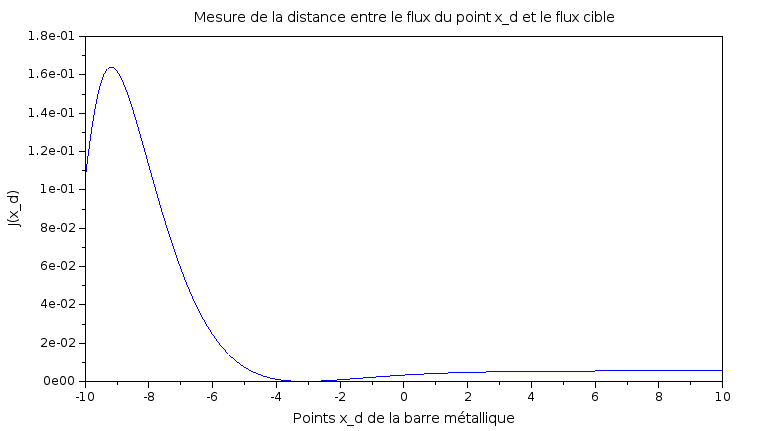
\includegraphics[scale=0.62]{images/q12_mesure_xd.png}
    \end{center}

    La fonction $J$ admet un unique minimum. C'est le flux égal au flux
    cible pour $x_d \simeq -3.5$. On implémente désormais deux méthodes pour
    trouver par le calcul cette valeur $x_d^{*}$ : la méthode de la dichotomie
    et la méthode de Gauss-Newton.\newline

    \bigskip
    \quest{QUESTION 13}. Méthode de la dichotomie.
    \begin{ref_scilab}
        \raisebox{-0.5ex}{
\includegraphics[height=12px]{images/logo_scilab.png}}
        \emph{Se référer à :} \texttt{\emph{Q13\_J\_Dichotomie.sce}}
    \end{ref_scilab}

    $J(x_d)$ est une mesure de la distance entre le flux en $x_d$ et le flux cible. On en déduit :

    \medskip
    \begin{algorithm}[H]
        \Donnees{$J(x_1), J(x_2), J(x_3)$}
        \Sortie{$I$, intervalle décidé}
        \uSi{$J(x_1) = \min(J(x_1), J(x_2), J(x_3))$}{$ I = \mathopen{[}a\,;x_2\mathclose{]}$}
        \uSinonSi{$J(x_2) = \min(J(x_1), J(x_2), J(x_3))$}{$ I = \mathopen{[}x_1\,;x_3\mathclose{]}$}
        \Sinon{$ I = \mathopen{[}x_2\,;b\mathclose{]}$}
    \end{algorithm}

    \newpage En effet, avoir $J(x_1)$ pour minimum signifie que, parmi les bornes $x_i$
    dont on dispose, c'est $x_1$ qui est le plus près de $x_d^{*}$. Cela nous assure que
    $x_d^{*}$ est entouré des mêmes bornes que $x_1$, ici $a$ et $x_2$. Le raisonnement
    est analogue pour les deux autres cas.\newline

    On affiche ici pour quelques itérations l'effet de la dichotomie sur l'intervalle
    de décision de départ et on constante qu'il se resserre
    autour de $x_d^{*}$ : $\mathopen{[}-6\,;3\mathclose{]}$.

    \begin{center}
        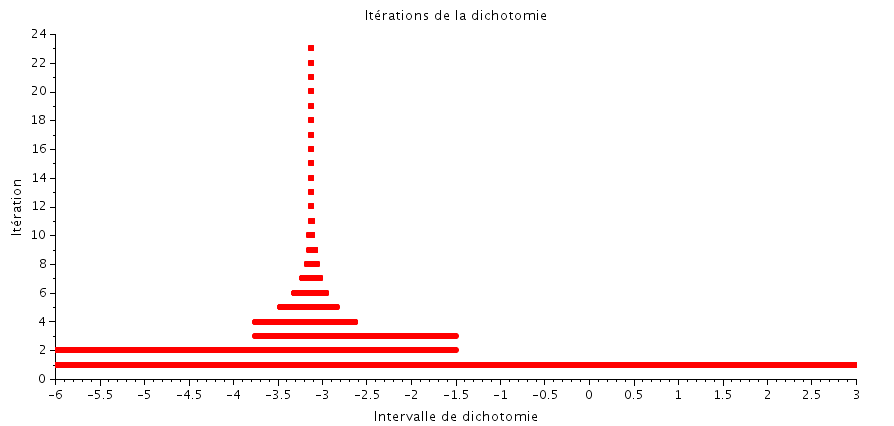
\includegraphics[scale=0.52]{images/q13_dichotomie.png}
    \end{center}

    \vspace{-2ex}
    \begin{calculs}
        \emph{Le résultat obtenu avec les données de l'énoncé est : \texttt{-3.12079}.}
    \end{calculs}

    \medskip
    \bigskip
    \quest{QUESTION 14}. Méthode de Gauss-Newton.
    \begin{ref_scilab}
        \raisebox{-0.5ex}{
\includegraphics[height=12px]{images/logo_scilab.png}}
        \emph{Se référer à :} \texttt{\emph{Q14\_J\_GaussNewton.sce}}
    \end{ref_scilab}

    La méthode de Gauss-Newton converge plus rapidement que la méthode dichotomique
    employée à la question précédente. En prenant $x_0 = 0$, on obtient ainsi le résultat
    à une précision de $10^{-5}$ avec les itérations suivantes :

    \begin{center}
        \begin{tabular}{|c|c|}
            \hline
            Itération & Valeur de $x_d$ \\
            \hline
            0 & \hspace{8ex}-6.55556\hspace{8ex} \\
            \hline
            1 & \hspace{8ex}-4.24829\hspace{8ex} \\
            \hline
            2 & \hspace{8ex}-3.31776\hspace{8ex} \\
            \hline
            3 & \hspace{8ex}-3.12891\hspace{8ex} \\
            \hline
            4 & \hspace{8ex}-3.12084\hspace{8ex} \\
            \hline
            5 & \hspace{8ex}-3.12079\hspace{8ex} \\
            \hline
        \end{tabular}
    \end{center}

    Six calculs de flux suffisent pour trouver $x_d^{*}$.
    Les bonnes propriétés de cette méthode dans notre
    cas peuvent s'expliquer par le fait que $x_0$ est initialisé près du minimum et
    que la fonction $J$ a une allure convexe sur un intervalle
    assez large autour de $x_d^{*}$ et $x_0$.

    \begin{calculs}
        \emph{Le résultat obtenu avec les données de l'énoncé est : \texttt{-3.12079}.}
    \end{calculs}
\end{document}
